\chapter{数据优化}
\label{cha:Database}
在WEB应用的开发和使用过程中,数据对于应用的价值越来越重要,因此在应用的使用过程中,保证数据库的正常工作以及数据的完整性将成为开发过程中数据库优化的主要目标。

目前应用开发过程中使用的数据库是MySQL,MySQL是一个开源的关系数据库管理系统,通过关系模型为用户提供数据的存储和修改等操作。

最新的稳定版为5.7.17,项目所使用的MySQL版本为5.7.11。较之前的版本,5.7版本的主要改进包括:
\begin{enumerate}
    \item 提升安全性

    为了增强数据库数据的安全性,在完成MySQL安装时,默认的root密码不再为空,而是随机生成一个密码,用户可以通过随机密码登录MySQL后修改密码。除此之外,新版本删除了test数据库,并且对用户创建的test数据库的权限进行了控制,同时提供了更为简单SSL安全访问配置,对于用户的密码可以设置有效期策略,超过有效期是强制用户修改密码来提升数据库安全,新版本还新增了对用户的暂时禁用功能。
    \item 增强数据存储的灵活性

    新版本在提升数据存储的灵活性方面增加了JSON和generate column两个新功能。

    随着非结构化数据存储需求的持续增长,各种非结构化数据存储的数据库应运而生(如MongoDB)。从最新的数据库使用排行榜来看,MongoDB已经超过了PostgreSQL,其火热程度可见一斑。各大关系型数据库也不甘示弱,纷纷提供对JSON的支持,以应对非结构化数据库的挑战。MySQL数据库从5.7.8版本开始,也提供了对JSON的支持。使用方式如下:
\begin{lstlisting}[language=sql,numbers=none]
CREATE TABLE t1 (jdoc JSON);
INSERT INTO t1 VALUES('{"key1": "value1", "key2": "value2"}');
\end{lstlisting}
MySQL对支持JSON的做法是,在server层提供了一堆便于操作JSON的函数,至于存储,就是简单地将JSON编码成BLOB,然后交由存储引擎层进行处理,也就是说,MySQL 5.7的JSON支持与存储引擎没有关系,MyISAM 存储引擎也支持JSON 格式。

MySQL支持JSON以后,总是避免不了拿来与MongoDB进行一些比较。但是,MySQL对JSON的支持,至少有两点能够完胜MongoDB:
\begin{enumerate}
\item 可以混合存储结构化数据和非结构化数据,同时拥有关系型数据库和非关系型数据库的优点
\item 能够提供完整的事务支持
\end{enumerate}

generated column是MySQL 5.7引入的新特性,所谓generated column,就是数据库中这一列由其他列计算而得。
\item 提升数据库运行的易用性

在开发或者运维人员进行数据库使用和状态检查的过程中,MySQL 5.7可以explain一个正在运行的SQL,这对于DBA分析运行时间较长的语句将会非常有用,同时performance\_schema提供了更多监控信息,包括内存使用,MDL锁,存储过程等。

除此之外,MySQL 5.7.7中引入了一个系统库sys schema,它包含了一系列视图、函数和存储过程, 该项目专注于MySQL的易用性。例如,我们可以通过sys schema快速的知道,哪些语句使用了临时表,哪个用户请求了最多的io,哪个线程占用了最多的内存,哪些索引是无用索引等

sys schema中包含了大量的视图,那么,这些视图的信息来自哪里呢?视图中的信息均来自performance schema统计信息。也就是说,performance schema提供了信息源,但是,没有很好的将这些信息组织成有用的信息,从而没有很好的发挥它们的作用。而sys schema使用performance schema信息,通过视图的方式给出解决实际问题的答案。

例如,下面这些问题,在MySQL 5.7之前,需要借助外部工具才能知道,在MySQL 5.7中,直接查询sys库下相应的表就能得到答案:
\begin{lstlisting}[language=sql,numbers=none]
# 如何查看数据库中的冗余索引
select * from sys.schema_redundant_indexes;
# 如何获取未使用的索引
select * from schema_unused_indexes;
# 如何查看使用全表扫描的SQL语句
select * from statements_with_full_table_scans
\end{lstlisting}
\item 提升了数据库的可用性

在以往的版本中,许多数据库的设置修改都需要重启服务使配置生效,在5.7版本中增加了许多改进,可以时一些必要的配置无需重启服务即可生效。

在线设置复制的过滤规则不再需要重启MySQL,只需要停止SQL thread,修改完成以后,启动SQL thread。

在线开启GTID,在之前的版本中,由于不支持在线开启GTID,用户如果希望将低版本的数据库升级到支持GTID的数据库版本,需要先关闭数据库,再以GTID模式启动,所以导致升级起来特别麻烦。MySQL 5.7以后,这个问题不复存在。

在线修改buffer pool的大小,MySQL 5.7为了支持online buffer pool resize,引入chunk的概念,每个chunk默认是128M,当我们在线修改buffer pool的时候,以chunk为单位进行增长或收缩。这个参数的引入,对innodb\_buffer\_pool\_size的配置有了一定的影响。innodb要求buffer pool size是innodb\_buffer\_pool\_chunk\_size* innodb\_buffer\_pool\_instances的倍数,如果不是,将会适当调大innodb\_buffer\_pool\_size,以满足要求,因此,可能会出现buffer pool的实际分配比配置文件中指定的size要大的情况.

Online DDL MySQL 5.7支持重命名索引和修改varchar的大小,这两项操作在之前的版本中,都需要重建索引或表.
\begin{lstlisting}[language=sql,numbers=none]
ALTER TABLE t1 ALGORITHM=INPLACE, CHANGE COLUMN c1 c1 VARCHAR(255);
\end{lstlisting}

\item 性能相关的改进
\begin{itemize}
\item 只读事务性能改进

众所周知,在传统的OLTP应用中,读操作远多于写操作,并且,读操作不会对数据库进行修改,如果是非锁定读,读操作也不需要进行加锁。因此,对只读事务进行优化,是一个不错的选择。

MySQL 5.6中,已经对只读事务进行了许多优化。例如,将MySQL内部实现中的事务链表分为只读事务链表和普通事务链表,这样在创建ReadView的时候,需要遍历事务链表长度就会小很多。

在MySQL 5.7中,首先假设一个事务是一个只读事务,只有在该事务发起了修改操作时,才会将其转换为一个普通事务。MySQL 5.7通过避免为只读事务分配事务ID,不为只读事务分配回滚段,减少锁竞争等多种方式,优化了只读事务的开销,提高了数据库的整体性能。
\item 加速连接处理

在MySQL 5.7之前,变量的初始化操作(THD、VIO)都是在连接接收线程里面完成的,现在将这些工作下发给工作线程,以减少连接接收线程的工作量,提高连接的处理速度。这个优化对那些频繁建立短连接的应用,将会非常有用。
\item 复制性能的改进

MySQL的复制延迟是一直被诟病的问题之一,欣喜的是,MySQL 5.7版本已经支持”真正”的并行复制功能。MySQL 5.7并行复制的思想简单易懂,简而言之,就是”一个组提交的事务都是可以并行回放的”,因为这些事务都已进入到事务的prepare阶段,则说明事务之间没有任何冲突(否则就不可能提交)。 经过对比测试,MySQL 5.7采用新的并行复制后,仍然会存在一定程度的延迟,只不过相比5.6版本减少了86\%,相比MariaDB的并行复制延迟也小不少。复制延迟问题得到极大改善。

除此之外复制性能的改进还包括多源复制,多从线程增强,在线 GTIDs,和增强的半同步复制等功能,这些功能均为保证数据的完整性可有效性提高了保障。
\end{itemize}
\end{enumerate}

存储引擎是存储数据、为存储的数据建立索引以及更新、查询数据等技术的实现方法。因为在关系数据库中数据的存储是以表的形式存储,所以存储引擎也可以称为表类型~\cite{胡雯2012mysql}。

Oracle和SQL Server等数据库中只有一种存储引擎,所有数据存储管理机制都一样。而MySQL数据库提供了多种存储引擎。用户可以根据不同的需求为数据表选择不同的存储引擎,用户也可以根据具体的需求编写自定义存储引擎。MySQL数据库提供的存储引擎如表~\ref{tab:mysql-engine}所示。

\begin{table}[H]
  \centering
  \begin{minipage}[t]{0.8\linewidth} % 如果想在表格中使用脚注,minipage是个不错的办法
  \caption[MySQL]{MySQL数据库存储引擎}
  \label{tab:mysql-engine}
    \begin{tabularx}{\linewidth}{lX}
      \toprule[1.5pt]
      {\heiti 存储引擎} & {\heiti 描述}\\\midrule[1pt]
      InnoDB  &  支持事务和行级锁,是Mysql上唯一一个提供了外键约束的引擎  \\
      MyISAM  &  基于ISAM存储引擎,常用的引擎,但是不支持事务、行级锁、而且崩溃后不能保证完全恢复。  \\
      ARCHIVE  &  仅支持插入和查询以及索引功能,拥有很好的压缩机制,适用于存储日志信息或其他按时间序列实现的数据采集类的应用场景中  \\
      CSV & 将数据文件保存为CSV格式的的文件,可以方便的导入到其他数据库中去,但是不支持索引 \\
      BLACKHOLE & 没有存储机制,任何数据都会被丢弃,但是会记录二进制日志\\
      FEDERATED & 可以访问远程服务器上数据的存储引擎,所以说它不再本地创建数据只会自动的建立一个连接到其他服务器上链接,有点类似于代理的功能\\
      MEMORY & 使用存储在内存中的内存来创建表,而且所有数据保存在内存中,数据安全性很低,但是查找和插入速度很快,通常用于临时表\\
      MRG\_MYISAM & 将多个MyISAM合并为一个\\
      \bottomrule[1.5pt]
    \end{tabularx}
  \end{minipage}
\end{table}

这些数据引擎中使用最广泛的是 MyISAM 和 InnoDB 两种存储引擎。MyISAM 是 MySQL 早期的ISAM存储引擎的升
级版本,也是 MySQL 默认的存储引擎,而 InnoDB 是由第三方软件公司 Innobase 所开发,其最大的特点是提供事务控制的特性~\cite{fruhwirt2010innodb}。

相比MyISAM,InnoDB数据引擎具有支持事务、行级锁和外键约束等功能。

\begin{enumerate}
\item 支持事务安全。InnoDB存储引擎最重要的一点就是对事务安全的支持,这也是让它成为最流行的存储引擎很重要的原因,而且实现了SQL92标准所定义的4个级别(READ UNCOMMITTED, READ COMMITTED, REPEATABLE READ, SERIALIZABLE).
\item 数据库多版本读取。InnoDB在事务支持的同时,为了保证数据的一致性以及并发时刻的性能,通过对un-do信息的聚簇索引实现对数据的多版本读取。
\item 锁定机制的改进。InnoDB改变了MyISAM的锁机制,实现了行锁。虽然InnoDB的行锁机制是通过索引来完成的,但是由于数据库中99\%的 SQL 语句都是通过索引来检索数据,所以行锁机制为InnoDB在承受高并发下的环境下增强了竞争力。
\item 实现外键。InnoDB实现了外键引用这一数据库的重要特性,使得在数据库端控制部分数据的完整性成为可能。
\end{enumerate}

\section{InnoDB引擎参数优化}

目前来说,InnoDB是为Mysql处理巨大数据量时的最大性能设计。它的CPU效率可能是任何其它基于磁盘的关系数据库引擎所不能匹敌的。在数据量大的网站或是应用中Innodb是倍受青睐的。另一方面,在数据库的复制操作中Innodb也是能保证master和slave数据一致有一定的作用~\cite{schwartz2012high}。由于InnoDB数据引擎在事务安全、支持外键以及数据恢复成本的综合性能表现,本论文中的WEB应用数据存储引擎使用的是InnoDB引擎。

为了保证在使用InnoDB引擎过程中,使WEB应用的数据稳定性和服务器负载达到最优的使用体验,还需要基于目前的WEB开发架构和服务器现状对MySQL的配置进行一定的参数调优。优化主要包括内存、IO、日志以及其它方面。

\begin{enumerate}
\item 内存利用方面

在内存利用方面,innodb\_buffer\_pool\_*相关的参数主要负载调控数据库在运行过程中数据缓存到内存的数据。其中innodb\_buffer\_pool\_size是InnoDB最重要的一个配置参数,主要缓存innodb表的索引,数据,插入数据时的缓冲。为Innodb加速优化首要参数。参数的默认分配只有8M,如果在配置过程中不调整这个值的话,会导致数据库的性能体验过差。

除此之外,还可以通过调整innodb\_buffer\_pool\_instances 来修改数据库缓冲池的实例数量,通过开启多个内存缓冲池,把需要缓冲的数据hash到不同的缓冲池中,这样可以并行的内存读写,在高IO负载时保持非常稳定的吞吐。

一般来说pool size参数和pool instance参数之前相互配置,通过不断的测试来调优二者的值,最终使数据库的内存利用方面达到最高。
\item IO控制方面

对于数据库的空间占用,可以通过修改innodb\_file\_*参数来配置,考虑到阿里云的磁盘扩展和读取的性能,这个参数的配置对于数据库的的性能提升效果不明显,因此没有必要做配置。

对于数据的IO分配来说,需要进行一定的优化,可以通过innodb\_file\_format配置文件的格式,提升存储数据的压缩比,可以通过修改innodb\_thread\_concurrency参数来配置线程的并发数,提升效率。
\item 日志控制方面

通过修改innodb\_log\_file\_size参数可以调整每个日志文件的大小,这个值分配的大小和数据库的写入速度,事务大小,异常重启后的恢复有很大的关系,由于当前的数据库服务器是阿里云数据库,硬盘为高速硬盘,数据的存取效率和IO压力均表现良好,故这个参数对于当前项目来说没有优化的必要。

通过修改innodb\_log\_buffer\_size参数可以日志缓冲区的大小,这个值分配的大小与内存中缓存的日志大小很大的关系,适当修改这个值可以降低内存的压力。

除了正常的日志外,InnoDB还有undo log,它记录某数据被修改前的值,可以用来在事务失败时进行回滚,因此通过调整undo log的相关参数可以在很大程度上保证数据的有效性。通过修改innodb\_undo\_log\_truncate参数值为1来开启在线回收undo 日志文件,通过修改innodb\_max\_undo\_log\_size参数值来配置触发回收undo 日志的阈值,通过innodb\_purge\_rseg\_truncate\_frequency参数来配置回收undo 日志的频率。
\item 其它方面优化

除了以上三个方面的优化之外,还有许多优化项目可以应用于本项目的数据库优化中。考虑到阿里云磁盘的性能,可以通过innodb\_flush\_method参数将数据和日志文件不经过缓存直接写入到文件中;通过innodb\_strict\_mode参数开启严格模式,对于写法错误的SQL语句跳过警告直接提示错误,提升数据库的稳定性;通过脏页的相关配置参数调整数据库对于脏页的刷新方式和效率,提升数据的有效性。
\end{enumerate}
综合以上各个方面的优化之后,本论文中WEB应用的数据库InnoDB引擎优化参数为:
\begin{lstlisting}[language=sql,numbers=none]
# 缓冲池字节大小
innodb_buffer_pool_size = 800M
# 缓冲池实例数量
innodb_buffer_pool_instances = 8
# 启动时将热数据加载到内存
innodb_buffer_pool_load_at_startup = 1
# 关闭时将热数据dump到本地磁盘
innodb_buffer_pool_dump_at_shutdown = 1
# page cleaner线程每次刷新脏页的数量
innodb_lru_scan_depth = 2000
# 事务等待获取资源等待的最长时间
innodb_lock_wait_timeout = 5
# 调整刷新脏页的数量
innodb_io_capacity = 4000
# 刷新脏页的最大值
innodb_io_capacity_max = 8000
# 数据和日志写入磁盘的方式-直接写入磁盘
innodb_flush_method = O_DIRECT
# 文件格式,Barracuda支持压缩页,新格式
innodb_file_format = Barracuda
# 设置文件格式最高版本
innodb_file_format_max = Barracuda
# 刷新脏页临近页
innodb_flush_neighbors = 1
# 用来缓冲日志数据的缓冲区大小
innodb_log_buffer_size = 1M
# 单独的清除线程数量-0不适用单独线程
innodb_purge_threads = 4
# 为字段创建索引时,限制的字节长度,超过直接报错
innodb_large_prefix = 1
# 线程并发数
innodb_thread_concurrency = 64
# 将发生的所有死锁信息都记录到错误日志中
innodb_print_all_deadlocks = 1
# 严格检查模式,写法有错误直接报错,不警告
innodb_strict_mode = 1
# 建立索引时用于排序数据的排序缓冲区大小-10M
innodb_sort_buffer_size = 10485760
# 转储缓冲池中read out and dump 的最近使用的页的占比
innodb_buffer_pool_dump_pct = 40
# page cleaner线程数量
innodb_page_cleaners = 4
# 开启在线回收undo log日志文件
innodb_undo_log_truncate = 1
# 超过这个阈值时触发回收
innodb_max_undo_log_size = 2G
# 回收undo日志的频率
innodb_purge_rseg_truncate_frequency = 128
\end{lstlisting}

\section{主从复制和延迟复制优化}
除了通过InnoDB引擎的配置来保证数据的有效性和稳定性之外,在数据库的开发是使用过程中还可以通过配置主从复制和延迟复制来保证数据。在5.7以前的MySQL版本中,由于主从复制的延迟问题,通常会选择第三方工具来进行数据的同步,但是通过第三方工具,对于数据同步的问题性由带来了问题,这些问题一直是运维人员在数据库开发过程中比较头疼的问题。随着5.7版本的发布,新版本在数据库主从复制方面进行了很多改进,包括降低了复制的延迟,通过looseless半同步方式提升了复制的稳定性。

MySQL数据库复制技术是把数据从一个数据库节点拷贝到其它一个或者多个数据库节点中,前者通常被称为主库(Master),后者通常被称为从库(Slave),如图\ref{fig:replication1}所示。
\begin{figure}[H] % use float package if you want it here
  \centering
  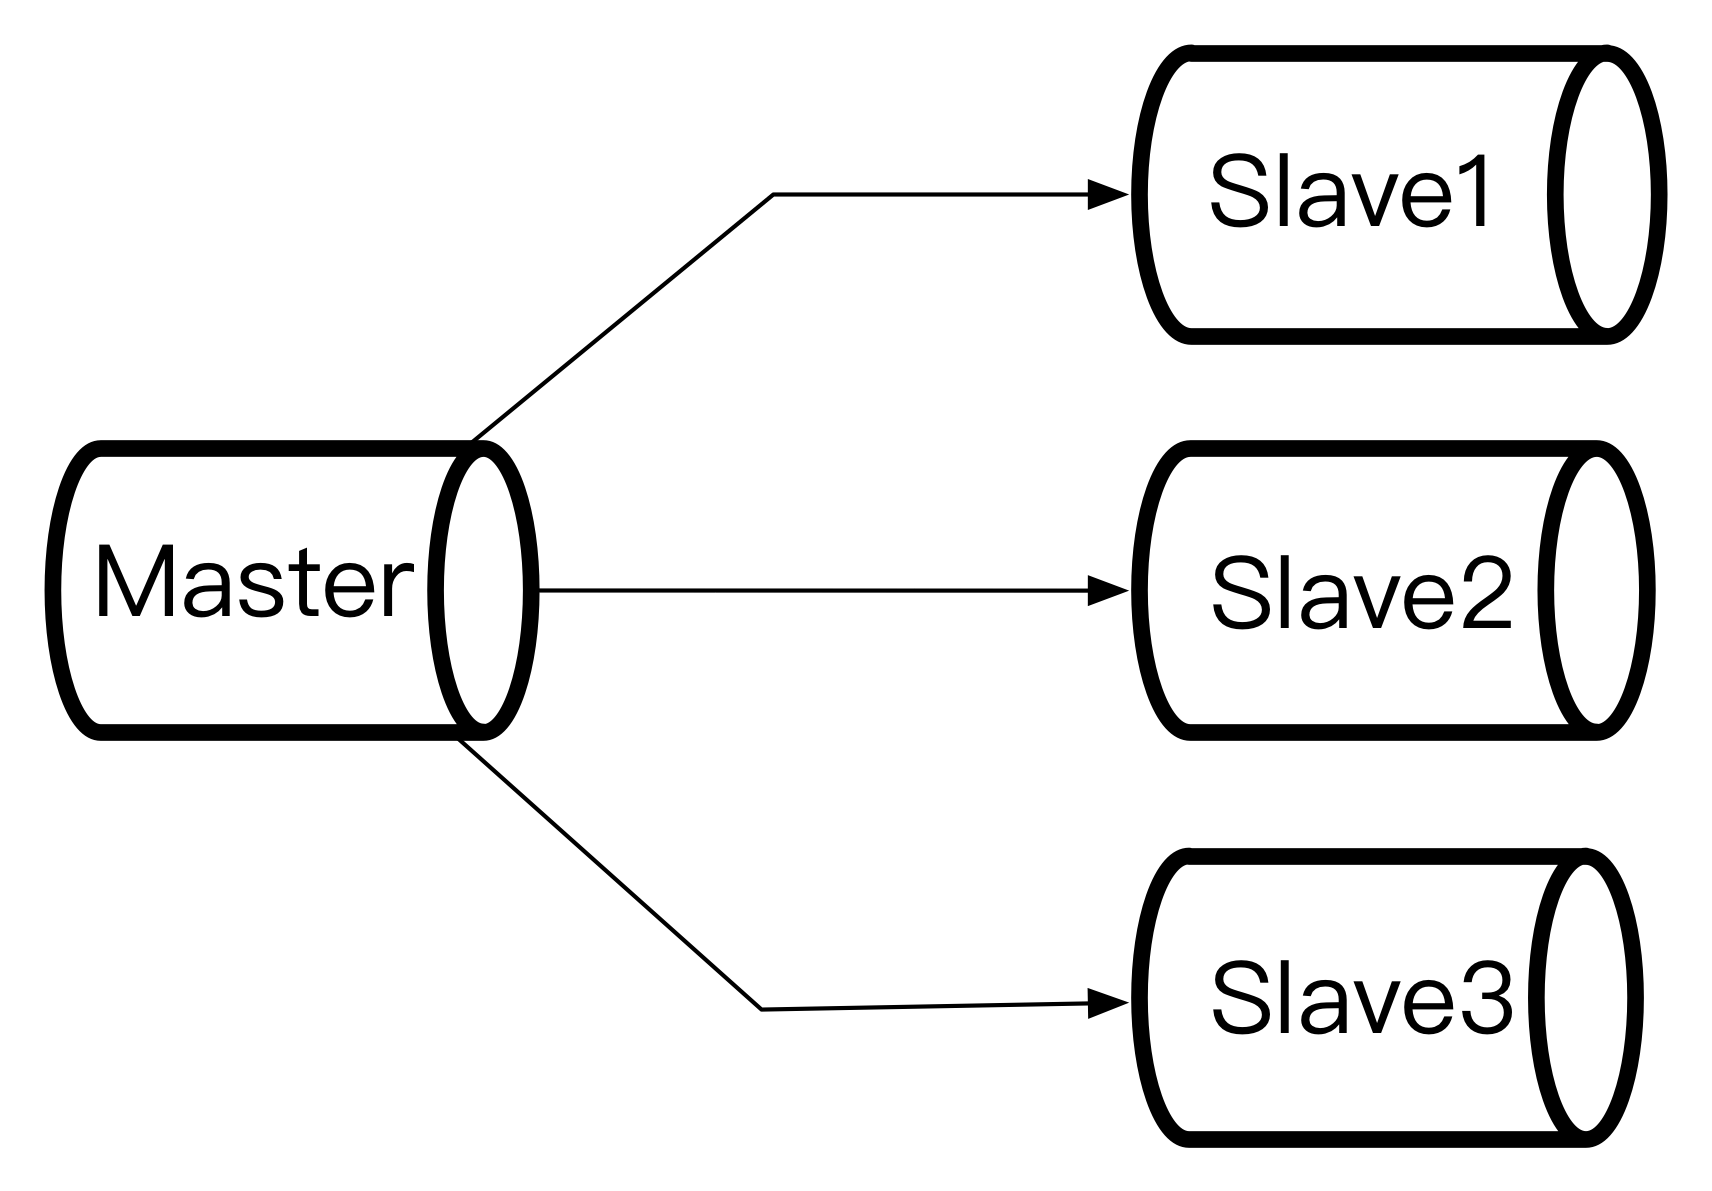
\includegraphics[width=3in]{chap04/replication1}
  \caption{MySQL复制示意图}
  \label{fig:replication1}
\end{figure}

复制的结果是集群(Cluster)中的所有数据库服务器得到的数据理论上都是一样的,都是同一份数据,只是有多个copy。MySQL默认内建的复制策略是异步的,基于不同的配置可以调整复制策略,Slave不一定要一直和Master保持连接不断的复制或等待复制,我们可以指定复制所有的数据库,一部分数据库,或者是某个数据库的某部分的表。

MySQL复制支持多种不同的复制策略,包括同步、半同步、异步和延迟策略等。
\begin{enumerate}
\item 同步策略:Master要等待所有Slave应答之后才会提交(MySql对DB操作的提交通常是先对操作事件进行二进制日志文件写入然后再进行提交)。
\item 半同步策略:Master等待至少一个Slave应答就可以提交。
\item 异步策略:Master不需要等待Slave应答就可以提交。
\item 延迟策略:Slave要至少落后Master指定的时间。
\end{enumerate}
MySQL复制同时支持多种不同的复制模式:
\begin{enumerate}
\item 基于语句的复制,Statement Based Replication(SBR)。
\item 基于行的复制Row Based Replication(RBR)。
\item 混合复制(Mixed)。
\end{enumerate}
使用MySQL复制,对于系统性能的提升主要表现在以下几个方面:
\begin{enumerate}
\item 性能方面:MySQL复制是一种Scale-out方案,也即“水平扩展”,将原来的单点负载扩散到多台Slave机器中去,从而提高总体的服务性能。在这种方式下,所有的写操作,当然包括UPDATE操作,都要发生在Master服务器上。读操作发生在一台或者多台Slave机器上。这种模型可以在一定程度上提高总体的服务性能,Master服务器专注于写和更新操作,Slave服务器专注于读操作,我们同时可以通过增加Slave服务器的数量来提高读服务的性能。

\item 防腐化:由于数据被复制到了Slave,Slave可以暂停复制进程,进行数据备份,因此可以防止数据腐化。

\item 故障恢复:同时多台Slave如果有一台Slave挂掉之后我们还可以从其他Slave读取,如果配置了主从切换的话,当Master挂掉之后我们还可以选择一台Slave作为Master继续提供写服务,这大大增加了应用的可靠性。

\item 数据分析:实时数据可以存储在Master,而数据分析可以从Slave读取,这样不会影响Master的性能。
\end{enumerate}
\subsection{数据库复制流程}
MySQL复制最常用的复制方式是通过二进制文件的方式进行复制,因此在配置数据库复制时,需要在主服务器和从服务器中开启二进制日志的配置。

复制的过程主要分为三步:
\begin{enumerate}
\item master将改变记录到二进制日志(binary log)中(这些记录叫做二进制日志事件,binary log events);
\item slave将master的binary log events拷贝到它的中继日志(relay log);
\item slave重做中继日志中的事件,将改变反映它自己的数据。
\end{enumerate}
图~\ref{fig:replication2}描述了复制的过程
\begin{figure}[H] % use float package if you want it here
  \centering
  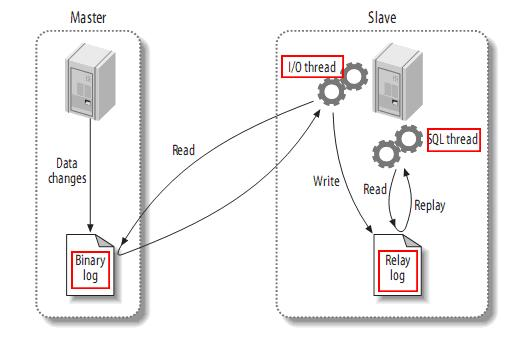
\includegraphics[width=3in]{chap04/replication2}
  \caption{MySQL复制流程}
  \label{fig:replication2}
\end{figure}
该过程的第一部分就是master记录二进制日志。在每个事务更新数据完成之前,master在二日志记录这些改变。MySQL将事务串行的写入二进制日志,即使事务中的语句都是交叉执行的。在事件写入二进制日志完成后,master通知存储引擎提交事务。

下一步就是slave将master的binary log拷贝到它自己的中继日志(relay log)。首先,slave开始一个工作线程——I/O线程。I/O线程在master上打开一个普通的连接,然后开始binlog dump process。Binlog dump process从master的二进制日志中读取事件,如果已经跟上master,它会睡眠并等待master产生新的事件。I/O线程将这些事件写入中继日志。

SQL slave thread处理该过程的最后一步。SQL线程从中继日志读取事件,更新slave的数据,使其与master中的数据一致。只要该线程与I/O线程保持一致,中继日志通常会位于OS的缓存中,所以中继日志的开销很小。

此外,在master中也有一个工作线程:和其它MySQL的连接一样,slave在master中打开一个连接也会使得master开始一个线程。复制过程有一个很重要的限制——复制在slave上是串行化的,也就是说master上的并行更新操作不能在slave上并行操作。

\subsection{双主复制设计}
目前生产环境的数据库有两个专有的服务器提供服务,为了保证数据的有效性,需要这两个服务器一个主服务器提供数据库的操作,另一个服务器作为从服务器,复制主数据库的数据。但是当主服务器出现问题而宕机时,需要快速的将从数据库切换为主数据库,在问题服务器恢复正常时作为从数据库,从新的主服务器复制数据。根据这个需求,将目前的两个数据库配置为双主数据库,将两个主数据库标示为master1和master2。

为了保证数据库的顺利复制,首先需要在两个数据库中通过stop slave命令来停止复制,并且保持两者的数据完全一致,通过reset master以及reset slave命令初始化。

然后在MySQl的配置文件中开启二进制日志,并为每一个数据库配置一个唯一的server-id,以及必要的配置。
\begin{lstlisting}[language=sql,numbers=none]
# 服务器ID
server-id = 1
# 开启二进制日志并配置日志名
log_bin = db2.bin
# 每一次事物提交都将binlog_cache中的数据强制写到磁盘
sync_binlog = 1
\end{lstlisting}
根据如上配置项,将两个数据库的二进制日志的文件名均配置为db2.bin,master1的server-id为1,master2的server-id为2,配置sync\_binlog参数为1表示每进行1次事务提交之后,MySQL将进行一次fsync之类的磁盘同步指令来将binlog\_cache中的数据强制写入磁盘,提高数据的持久性。

除此之外,需要在配置文件中开启GTID
\begin{lstlisting}[language=sql,numbers=none]
# 开启gtid工作模式
gtid_mode = on
# 只允许能保障事物安全,且能够被日志记录的SQL语句被执行
enforce_gtid_consistency = 1
# 从库从主库复制数据时的操作也写入binlog
log_slave_updates
# 重启和启动时,如何迭代使用binlog文件
binlog_gtid_simple_recovery = 1
完成基本配置后,需要在数据库中配置和连接master。
\end{lstlisting}
GTID是全局事务标识(global transaction identifieds),在数据库中一个事务对应一个GTID,而且一个GTID在一个服务器上只执行一次,避免重复执行导致数据混乱或者主从不一致,通过GTID可以保证日志文件中每一次事务都对应一个唯一的标志,对于从库拉取日志和日志分析具有很重要的意义。
\begin{enumerate}
\item 创建用于主从复制的用户
\begin{lstlisting}[language=sql,numbers=none]
GRANT REPLICATION SLAVE ON *.* TO 'repl'@'%' IDENTIFIED BY 'replpassword';
\end{lstlisting}
其中repl为用户名,replpassword为密码
\item 配置master信息
\begin{lstlisting}[language=sql,numbers=none]
change master to master_host ='ip', master_port = port, master_user = 'repl', master_password = 'replpassword', master_auto_position =1;
\end{lstlisting}
变量master\_host值为master所在服务器的IP地址,master\_port为master服务器的数据库连接端口,配置好用户名和密码。
master\_auto\_position让从库根据 GTID自动选择适当的事务点进行复制,基本上无需关注和担心主从不一致的问题。
\item 启动复制,并查看状态。
\begin{lstlisting}[language=sql,numbers=none]
start slave;
show slave status;
\end{lstlisting}
在查询结果的字段中通过Slave\_IO\_Running和Slave\_SQL\_Running两个变量的值为YES来判断主从复制是否成功启动。
\end{enumerate}

在master1和master2上均按照上述步骤进行操作,完成高可用的双主复制的部署。
\subsection{延迟复制设计}
为了避免上述双主服务器均出现问题后无法提供数据服务的现象,在测试服务器中搭建一个延时复制服务器,延时复制的主库配置为master1,将复制策略配置为延迟1小时复制,然后通过二进制日志进行近小时内数据的恢复,这样能够最大程度保证数据的完整。

配置的步骤基本类似于双主的配置,但是在配置master信息后需要增加一步,调整复制的延迟时间,单位是ms,因此一小时延时的变量值为3600。

\begin{lstlisting}[language=sql,numbers=none]
CHANGE MASTER TO MASTER_DELAY = 3600;
\end{lstlisting}

%\section{数据库负载均衡}
\section{数据库备份}
除了通过延迟复制来保证数据之外,服务器还将每天对数据库进行一次备份,并且将备份的数据库上传到阿里云的对象存储OSS中,目前master1和master2数据库的数据是一致的,因此只需要对master1的数据库进行备份即可。

备份通过mysqldump命令进行备份,备份完成之后通过阿里云OSS的Python SDK将备份文件上传到OSS中。

\begin{enumerate}
\item 开发OSS文件上传脚本

首先需要通过pip install oss2 命令在备份服务器中安装Python版本的OSS SDK,安装完成后在服务器的/mnt/sh中新建oss目录,并在oss目录下创建上传脚本dbuposs.py文件。修改文件如下:
\begin{lstlisting}[language=python]
#!/usr/bin/python2.7
# -*- coding: utf-8 -*-
import oss2
import sys
auth = oss2.Auth('AccessKeyId', 'AccessKeySecret ')
endpoint='http://oss-cn-beijing-internal.aliyuncs.com'
bucket = oss2.Bucket(auth, endpoint, 'mysqlbk')
bucket.put_object_from_file(sys.argv[1], '/mnt/mysqldump/'+sys.argv[1])
\end{lstlisting}
在脚本中配置阿里云OSS的访问域名(本项目的OSS访问域名为http://oss-cn-beijing-internal.aliyuncs.com),以及访问OSS的AccessKeyId和AccessKeySecret。配置完成之后即可完成访问OSS的认证工作。

通过oss2.Bucket函数连接OSS的mysqlbk存储空间获取bucket对象。

通过bucket对象的put\_object\_from\_file函数将指定的文件上传到OSS中,完成文件上传。
\item 开发数据库备份脚本

数据库脚本可以通过Bash脚本来实现,前提是需要在服务器中安装mysql,脚本的存放位置为/mnt/sh/mysqlbak.sh。

备份的流程主要为:首先要配置被备份数据库的相关信息,包括用户名、密码、端口、IP地址、数据库名称等变量;然后配置备份数据的保存位置和命名方式,以及日志的相关配置;之后通过执行mysqldump备份数据库到本地,通过tar命令将备份的sql文件压缩;最后通过调用OSS上传脚本将压缩后的备份文件上传到OSS中。同时,本地目录中只保存七天内的数据库备份文件,超过七天的文件会被删除。

备份脚本如下:
\begin{lstlisting}[language=bash]
#!/bin/bash
PATH=/bin:/sbin:/usr/bin:/usr/sbin:/usr/local/bin:/usr/local/sbin
export PATH
#数据库用户名
dbuser='root'
#数据库用密码
dbpasswd='password'
#需要备份的数据库,多个数据库用空格分开
dbname='minishop'
#备份时间
backtime= (date +%Y%m%d%H%M%S)
#日志备份路径
logpath='/mnt/mysqldump'
#数据备份路径
datapath='/mnt/mysqldump'
#日志记录头部
echo "备份时间为${backtime},备份数据库表 ${dbname} 开始" >> ${logpath}/log.log
#正式备份数据库
for dbn in $dbname; do
source=(mysqldump -u${dbuser} -p${dbpasswd} -hdbip -Pdbport ${dbn} --set-gtid-purged=OFF > ${logpath}/${backtime}.sql) 2>> ${logpath}/mysqllog.log;
#备份成功以下操作
if [ "$?" == 0 ];then
cd $datapath
#为节约硬盘空间,将数据库压缩
tar jcf ${dbn}${backtime}.tar.bz2 ${backtime}.sql > /dev/null
#删除原始文件,只留压缩后文件
rm -f ${datapath}/${backtime}.sql
#上传到oss
/mnt/sh/oss/dbuposs.py ${dbn}${backtime}.tar.bz2
#删除七天前备份,也就是只保存7天内的备份
find $datapath -name "*.tar.bz2" -type f -mtime +7 -exec rm -rf {} \; > /dev/null 2>&1
echo "数据库表 ${dbname} 备份成功!!" >> ${logpath}/mysqllog.log
else
#备份失败则进行以下操作
echo "数据库表 ${dbname} 备份失败!!" >> ${logpath}/mysqllog.log
fi
done
\end{lstlisting}

\item 定时任务设置
为了保证每天都进行一次数据库备份操作,需要通过定时任务来保证数据库备份脚本每天执行一次。在Linux环境中,通过crontab软件来执行定时任务。crontab是一个在类Unix操作系统上的任务计划程序,它可以让用户在指定时间段周期性地运行命令或者shell脚本,通常被用在系统的自动化维护或者管理。

在本项目中,cron定时任务的配置文件在/var/spool/cron中的root文件,在root文件中添加如下定时任务:
\begin{lstlisting}[language=sh,numbers=none]
#<分钟> <小时> <日> <月份> <星期> <命令>
00 00 * * * /mnt/sh/mysqlbak.sh
\end{lstlisting}
设定在每天的凌晨0点0份执行数据库备份脚本。
\end{enumerate}
%\section{数据恢复方案}
\section{本章总结}
本章是对本论文中WEB项目的数据库进行优化的一些策略,主要包括通过InnoDB配置参数调整提升数据库自身的运行性能,通过配置主从复制以及延迟复制提升数据的稳定性和有效性,通过开发数据库定时备份脚本来实现数据库的每日备份。通过这些策略,在提升MySQL运行性能同时也保证了数据的完整性和有效性,对于WEB应用的作用至关重要。